% -*- coding: utf-8; -*-
% vim: set fileencoding=utf-8 :

% The paper on using Luau telemetry to measure the effectiveness of type error reporting.

\documentclass[english,submission,cleveref]{programming}
%% use 'submission' for initial submission, remove it for camera-ready (see 5.1)

%%\overfullrule=1mm

%% BEGIN tobias pape 2021-11-06
\makeatletter
\newcommand*\abstractpart[1]{\unskip\par\noindent{\firamedium\color{P@GrayFG}{#1}}\enspace}
\makeatother
%% END

\usepackage{alltt}
\usepackage[backend=biber]{biblatex}
\usepackage{amssymb}
\usepackage{calc}
\usepackage{listings}
\usepackage{mathpartir}
\usepackage{pifont}
\usepackage{siunitx}
\usepackage{tikz}
\usepackage{subcaption}
\usepackage{wasysym}
\usepackage{xcolor}
\usetikzlibrary{shapes.geometric}

\addbibresource{bib.bib}

%%%%%%%%%%%%%%%%%%
\paperdetails{
  %% perspective options are: art, sciencetheoretical, scienceempirical, engineering.
  %% Choose exactly the one that best describes this work. (see 2.1)
  perspective=scienceempirical,
  %% State one or more areas, separated by a comma. (see 2.2)
  %% Please see list of areas in http://programming-journal.org/cfp/
  %% The list is open-ended, so use other areas if yours is/are not listed.
  area={Data mining for programming, Telemetry},
  %% You may choose the license for your paper (see 3.)
  %% License options include: cc-by (default), cc-by-nc
  % license=cc-by,
}
%%%%%%%%%%%%%%%%%%

%%%%%%%%%%%%%%%%%%
%% These data are provided by the editors. May be left out on submission.
%\paperdetails{
%  submitted=2023-1-31,
%  published=2016-10-11,
%  year=2016,
%  volume=1,
%  issue=1,
%  articlenumber=1,
%}
%%%%%%%%%%%%%%%%%%

\begin{document}

\title{Millions of Type Errors}
\subtitle{Impersonal Telemetry to Measure User Experience}
% lean, lite, modest, non-intrusive, private, ...

% Alphabetical order for authors?

\author[a]{Ben Greenman}
\authorinfo{(\email{benjamin.l.greenman@gmail.com}) is a postdoc at Brown University. He will be joining the University of Utah in Fall~2023.}
\affiliation[a]{Brown University, Providence, RI, USA}
% \orcid{0000-0001-7078-9287}
\affiliation[a]{Brown University, Providence, RI, USA}

\author[b]{Alan Jeffrey}
\authorinfo{(\email{ajeffrey@roblox.com}) TBD}
% \orcid{0000-0001-6342-0318}
\affiliation[b]{Roblox, San Mateo, CA, USA}

\author[a]{Shriram Krishnamurthi}
% \orcid{0000-0001-5184-1975}
\authorinfo{(\email{shriram@brown.edu}) is the Vice President of Programming Languages (no, not really) at Brown University.}

\author[b]{Mitesh Shah}
\authorinfo{(\email{mshah@roblox.com}) TBD.}

%\renewcommand{\shortauthors}{...}

\newcommand{\code}[1]{\texttt{#1}}
\newcommand{\FILL}{\textbf{FILL}}
\newcommand{\dotscale}[1]{\scalebox{0.72}{#1}}
\newcommand{\wideas}[2]{\makebox[\widthof{#2}][l]{#1}}
\newcommand{\twoline}[2]{\parbox[s]{1.4cm}{\flushleft#1\newline#2}}
\newcommand{\chkYes}{\dotscale{\CIRCLE}}
\newcommand{\chkMaybe}{\wideas{\dotscale{\Circle}}{\chkYes}}
\newcommand{\chkNo}{\wideas{}{\chkYes}}
\newcommand{\pct}[1]{\SI{#1}{\percent}}
\newcommand{\modefont}[1]{\texttt{#1}}
\newcommand{\mnocheck}{\modefont{nocheck}}
\newcommand{\mnonstrict}{\modefont{nonstrict}}
\newcommand{\mstrict}{\modefont{strict}}
\newcommand{\zerowidth}[1]{\makebox[0pt][l]{#1}}

%%
%% The code below is generated by the tool at http://dl.acm.org/ccs.cfm.
%% Please copy and paste the code instead of the example below.

\begin{CCSXML}
<ccs2012>
<concept>
<concept_id>10011007.10011006.10011039.10011311</concept_id>
<concept_desc>Software and its engineering~Semantics</concept_desc>
<concept_significance>500</concept_significance>
</concept>
<concept>
<concept_id>10011007.10011006.10011008.10011024.10011032</concept_id>
<concept_desc>Software and its engineering~Constraints</concept_desc>
<concept_significance>100</concept_significance>
</concept>
<concept>
<concept_id>10011007.10011006.10011008.10011009.10011012</concept_id>
<concept_desc>Software and its engineering~Functional languages</concept_desc>
<concept_significance>100</concept_significance>
</concept>
</ccs2012>
\end{CCSXML}

\ccsdesc[500]{Software and its engineering~Semantics}
\ccsdesc[100]{Software and its engineering~Constraints}
\ccsdesc[100]{Software and its engineering~Functional languages}

\keywords{types, gradual typing, telemetry, user study, large-scale study}

\maketitle

\begin{abstract}
  {Roblox Studio} is a tool which places programming in the hands of
  millions of creators, ranging from high school students to professional
  development studios. It has the ability to report telemetry data,
  which allows large-scale measurement of the creator experience. In
  this paper, we discuss one use of telemetry, to measure the experience
  of type error reporting.
  We find FILL.

  %\let\paragraph\abstractpart

  % \paragraph{Context}
  %% What is the broad context of the work? What is
  %% the importance of the general research area?

  % \paragraph{Inquiry}
  %% What problem or question does the paper
  %% address? How has this problem or question been
  %% addressed by others (if at all)?

  %\paragraph{Approach}
  %% What was done that unveiled new knowledge?

  %\paragraph{Knowledge}
  %% What new facts were uncovered? If the
  %% research was not results oriented, what new
  %% capabilities are enabled by the work?

  %\paragraph{Grounding}
  %% What argument, feasibility proof, artifacts,
  %% or results and evaluation support this work?

  %\paragraph{Importance}
  %% Why does this work matter?

\end{abstract}

\section{Introduction}
\label{s:introduction}

{Roblox} is a platform for {shared virtual experiences},
with 56~million Daily Active Users, and 49~billion hours of engagement in
2022~\cite{roblox-quarterly-results}.
There are \textbf{XX}~million creators using {Roblox Studio},
and \textbf{YY}~million creations.

{Roblox experiences} are scripted using the 
{Luau} programming language~\cite{luau-lang.org},
an extension of {Lua~5.1~\cite{lua}}.
The main extension is the addition of a static type system, which uses
type inference to synthesize types for user code. These types
are used primarily in type-driven tooling such as autocomplete
and API documentation~\cite{luau-autocomplete},
but creators can also opt in to receiving type error reports.

As discussed in~\cite{bfj-hatra-2021},
the goals of the {Luau} type system are rather different from
a traditional type system, which focuses on compilation and memory safety.
{Luau} has a diverse user community, ranging from
students in code camps to professional development studios. These
creators have quite different needs, with different emphases on
enabling rapid creation and ensuring software quality.
{Luau} therefore supports three typing modes---strict types,
relaxed (nonstrict) types, and no types---and lets users switch
between modes gradually~\cite{st-sfp-2006,tfffgksst-snapl-2017}, one module at a time.

In this paper, we investigate methods for measuring the effectiveness
of the {Luau} type system in the development of {Roblox} scripts.
In comparison to prior work~(\cref{s:related}), which is either small in scale
or depends on personally identifiable information~(PII),
we performed a large-scale study using pseudonymized \emph{telemetry}.

{Roblox Studio} has a telemetry system, which is used to gauge
the effectiveness of creation features. This system stochastically
determines which sessions should report telemetry, and for those
sessions, reports telemetry records back with a summary of the
session. In the case of this study, the telemetry includes data on the
number of errors at various levels of granularity: in the current edit
range, in the current file, and in every file which was type
checked.

The telemetry data we analyzed does not contain any PII:
no source code;
no source code locations;
no error messages (which may contain source code);
no record of the creator's identity, locale, or IP address;
and no information about what creation the data came from.
Telemetry records are correlated by session, using a pseudonymized
session identifier.

Most users of {Roblox Studio} do not opt in to type error
reporting, and so they do not see the ``squiggly underlining'' that
indicates a type error site. Nonetheless, the type inference system
still runs in the background (since it drives autocomplete and other
type-based tools), letting us see which type errors would have
been reported and whether users fix these errors over time.

With this telemetry data, we investigate research questions about
the adoption and benefits of type analysis:
\begin{description}
  \item[RQ1.]
    How many creators use type analysis?
    How often do projects contain modules with different
    analysis modes?
    How often do creators turn analysis off?
  \item[RQ2.]
    For modules that use type analysis:
    which errors arise,
    how do creators respond,
    and which errors tend to persist despite subsequent edits?
  \item[RQ3.]
    What impact does type analysis have on the number of background type
    errors?
    For example, do background errors pile up in unanalyzed projects?
\end{description}

Beyond their immediate applications to {Lua},
answers to these questions have implications for the design
of gradual types, success types, and semantic subtyping.
Luau represents the first large-scale combination of these features,
and lessons from this experience can inform future applications.

At a higher level, this paper is the first to use telemetry 
to study a typechecker.
It thus represents a step toward data-driven language design,
informed by many users' actual practice.
Our data captures \textbf{XX} sessions
for a total of \textbf{YY} hours
and \textbf{ZZ} type errors.
By contrast to typical qualitative methods (e.g., surveys and interviews), it
is not restricted to users' \emph{perceptions} about their work and it is not
limited to a small number of users.

FILL can stats answer questions that point-by-point analysis cannot?

\paragraph{Contributions}
\begin{itemize}
  \item
    Design of a low-overhead, (black-box / PII-safe / impersonal)
    telemetry method, that other
    researchers can build on.

  \item
    Lessons from millions of type errors about
    the adoption of strict type analysis,
    the usefulness of type errors,
    and \FILL{}.
    These findings are especially important for the
    gradual typing, success typing, and semantic subtyping communities.

  \item
    \FILL{} any surprises when doing the analysis?
    Note, no ML for analysis, we do not have a corpus of text.

\end{itemize}

Analysis pipeline to be freely available.
Data may be available, depends on Roblox.


\section{{Roblox} Context}
% https://create.roblox.com/docs/scripting/luau

FILL table = object

\begin{figure}

  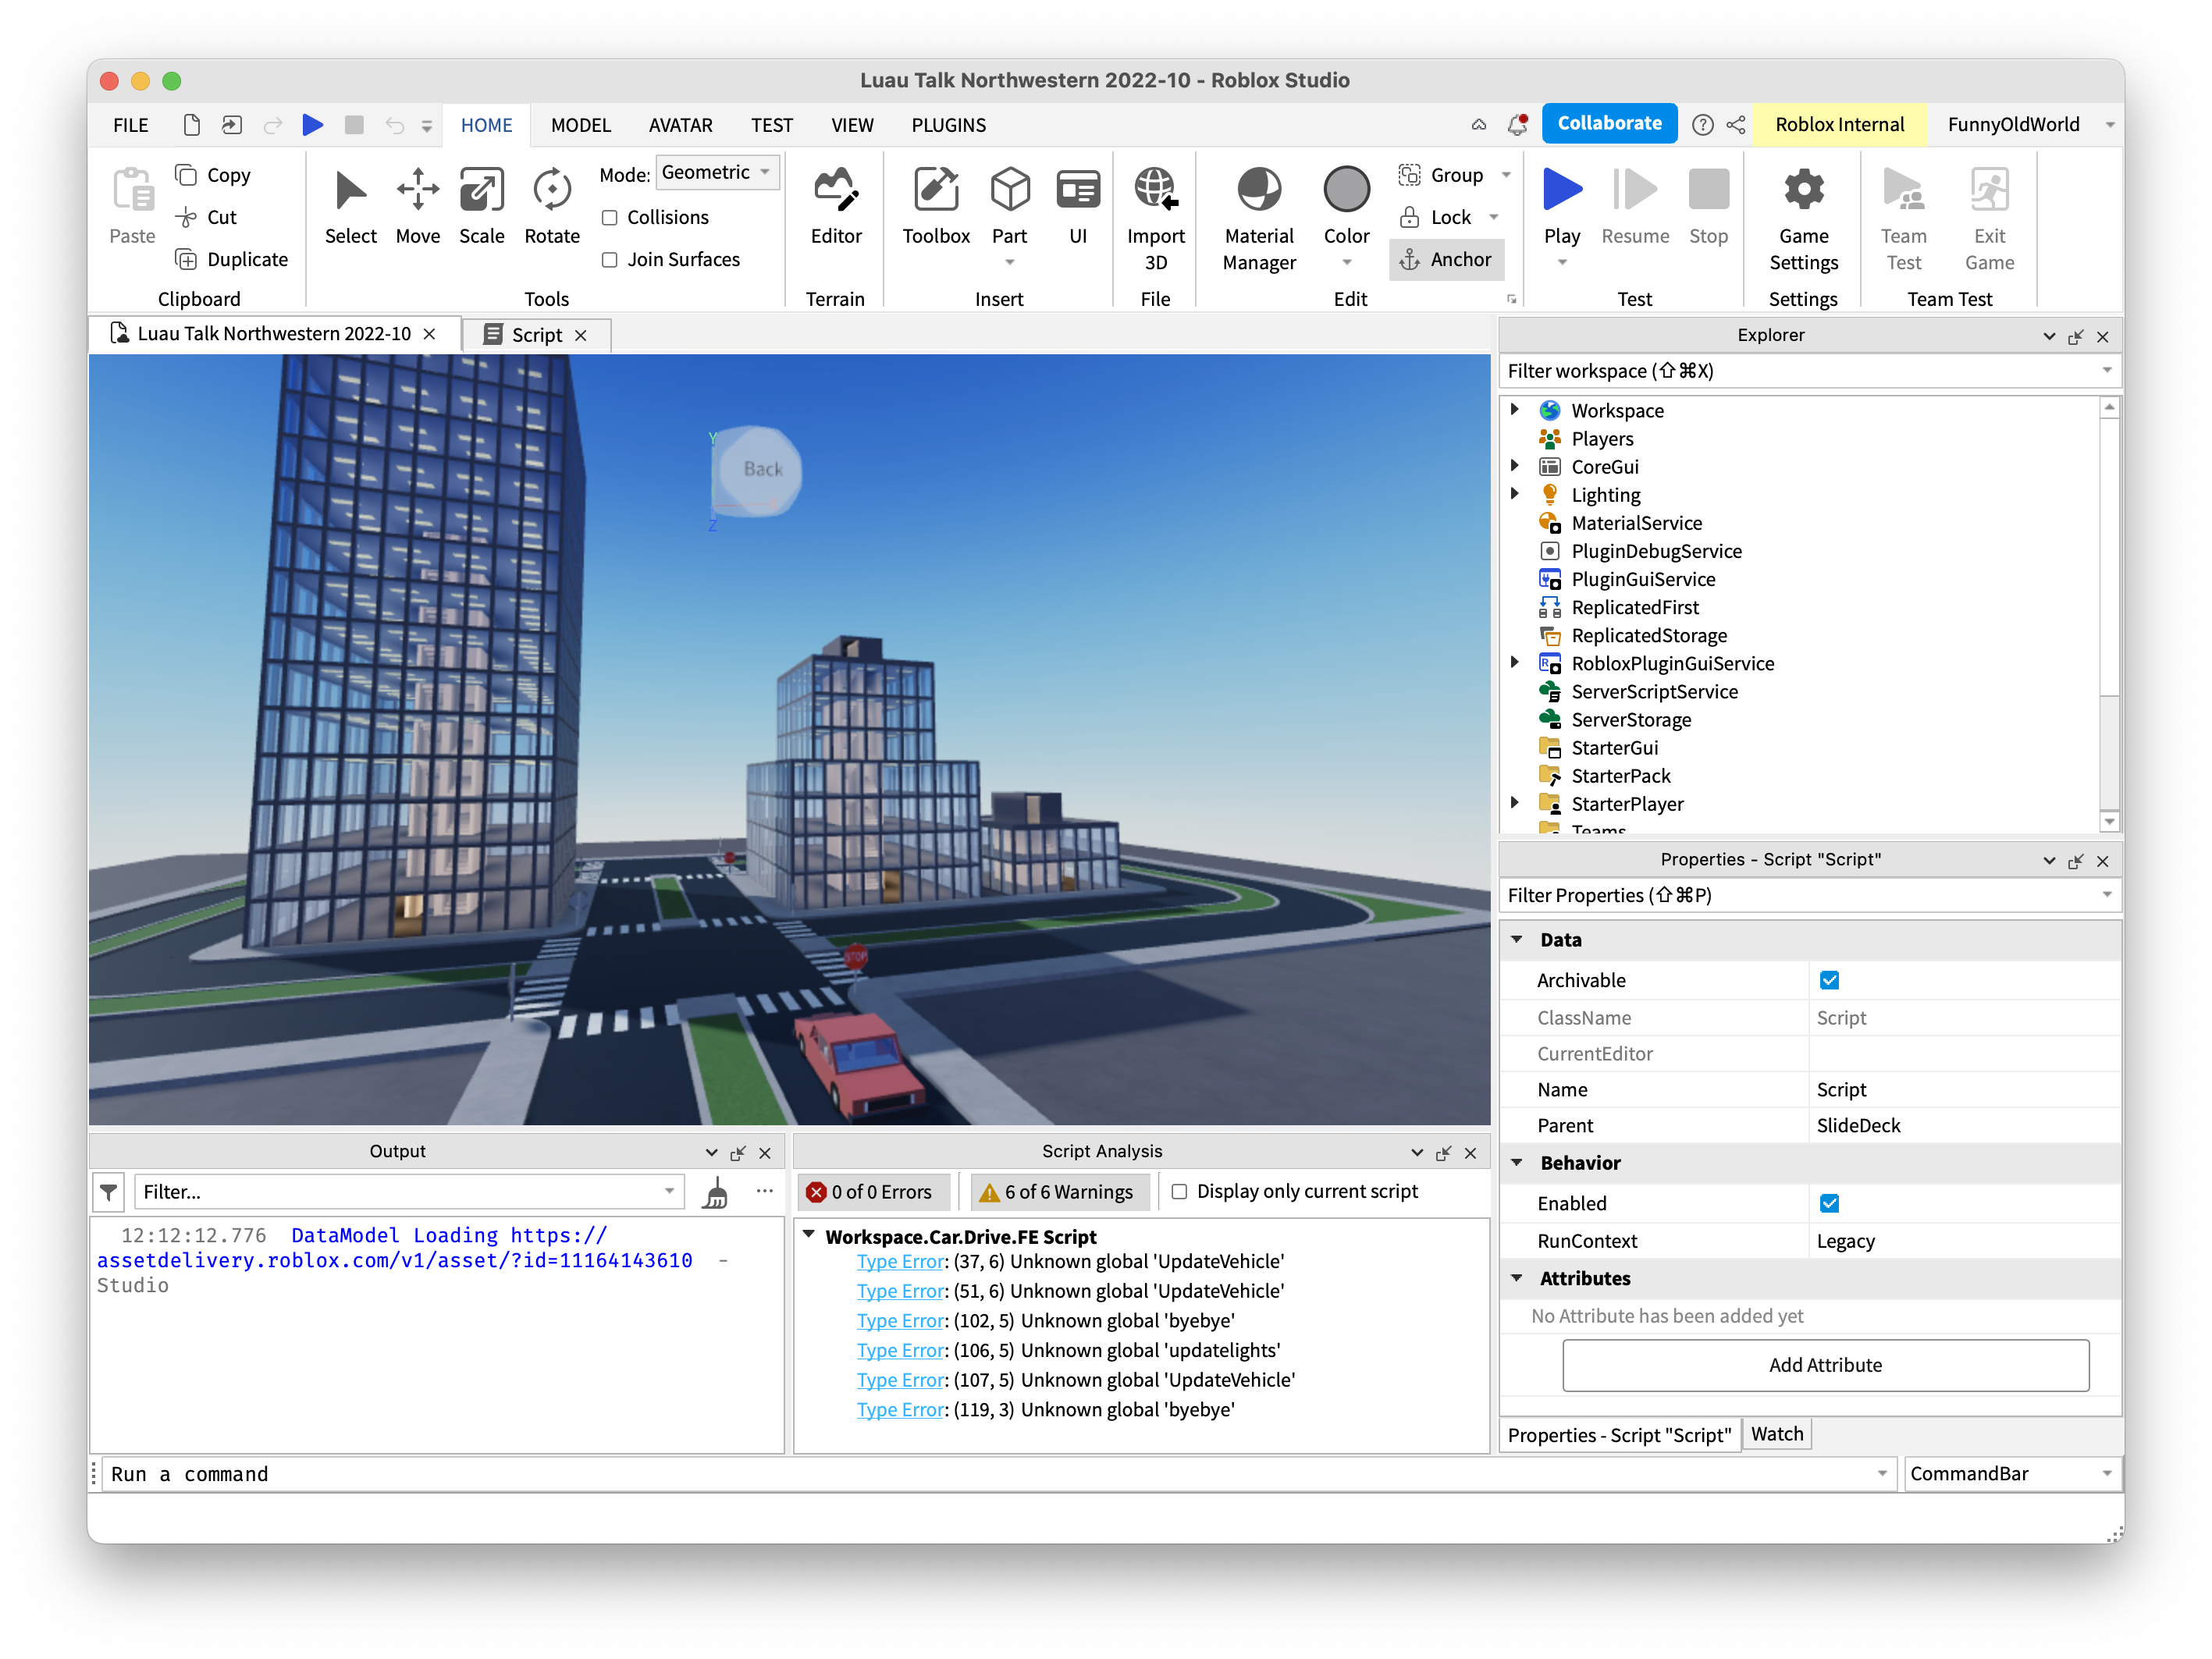
\includegraphics[width=.45\textwidth]{img/roblox-studio.png}
  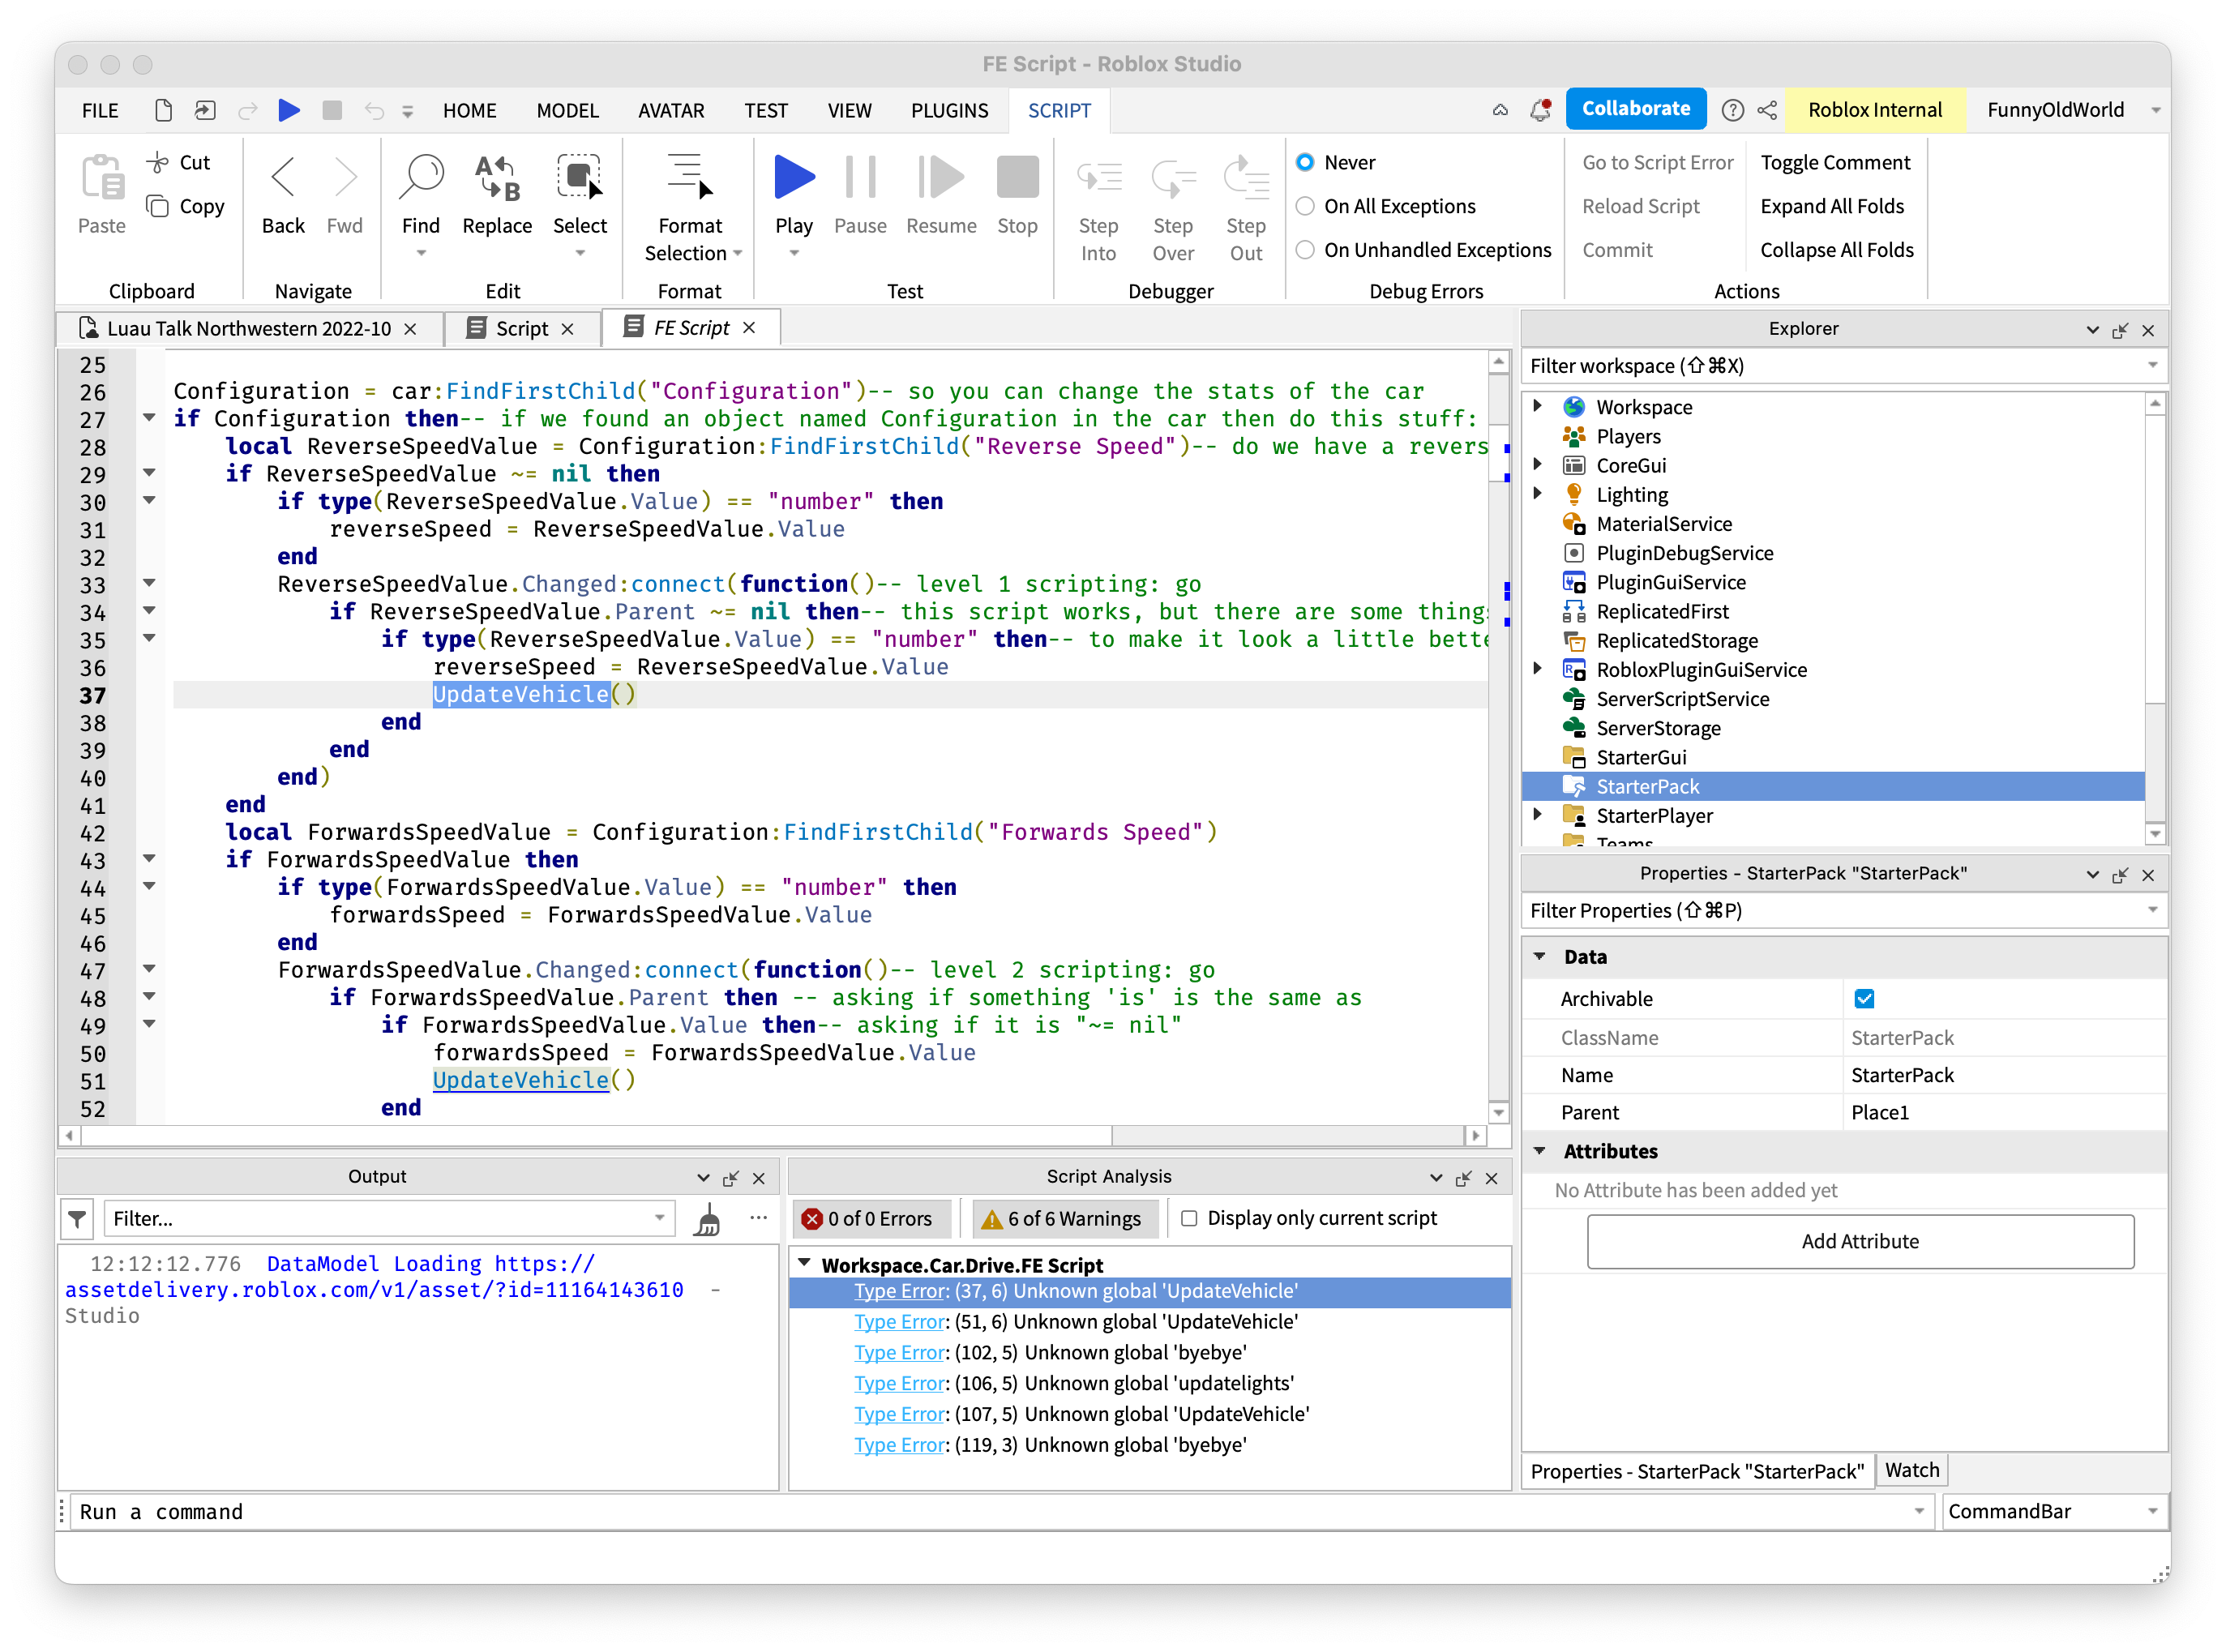
\includegraphics[width=.45\textwidth]{img/roblox-studio-ide.png}

  \caption{{Roblox Studio 3D creation} tools (left) and IDE (right)}
  \label{fig:roblox-studio}
\end{figure}

Creators of {Roblox experiences} use {Roblox Studio},
which combines {3D creation} tools as well as an Integrated
Developer Environment (IDE), as seen in Fig.~\ref{fig:roblox-studio}.
The IDE includes an optional ``Script Analysis'' widget, which
reports syntax errors, type errors, and problems identified by
lint tools. The script editor also (optionally) highlights
the location in code where reported errors occur.

To opt in to type error reporting, creators set a \emph{mode}
for each script, which is one of:
\begin{itemize}
  \item \mnocheck{}: only syntax errors are reported,
  \item \mnonstrict{}: all syntax errors, and a subset of ``high probability'' type errors, are reported, or
  \item \mstrict{}: all syntax errors and type errors, are reported.
\end{itemize}
As an example of nonstrict mode, the following program only reports one error:
\begin{verbatim}
--!nonstrict
local x = { p = 5, q = nil }
if condition then x.q = 7 end
local y = x.p + x.q --> no type error
local z = x.r       --> "Key 'r' not found in table 'x'"
\end{verbatim}
but in strict mode it reports two:
\begin{verbatim}
--!strict
local x = { p = 5, q = nil }
if condition then x.q = 7 end
local y = x.p + x.q --> "Type 'nil' could not be converted into 'number'"
local z = x.r       --> "Key 'r' not found in table 'x'"
\end{verbatim}
In cases like this, where it is undecidable whether there will be a run-time error,
strict mode errs on the side of reporting an error, and nonstrict mode errs on
the side of suppressing the error.

Both modes report the \verb|Key 'r' not found in table 'x'| error --
misspellings of property names are common enough to report in both
strict and nonstrict mode. See~\cite{bfj-hatra-2021}
for a more detailed discussion of the rationale for strict and nonstrict mode.

Both modes are opt-in. Creators have the option to make nonstrict mode
the default rather than \mnocheck{} mode.

Even in \mnocheck{} mode, {Roblox Studio} performs type inference, since
the results are needed by type-directed tooling such as autocomplete and
API documentation. This behind-the-scenes typechecking is always performed
in strict mode, since it is important that the inferred types be as precise
as possible. The type errors produced by this pass are always discarded,
so the verbosity of strict mode is not an issue.

Since this pass is always performed in strict mode, we refer to it as
\emph{forced strict} mode. Its main use is in autocomplete, so forced
strict mode is triggered on every keystroke

Scripts come in two favors: \emph{module scripts} and \emph{non-module
scripts}.  Module scripts provide reusable libraries, which may be
\emph{required} by other scripts. Since module scripts can require
other module script, modules form a graph (though we consider it to be
an error in strict mode if the graph is cyclic, and remove edges to
make it acyclic).

When typechecking is performed for script analysis, any script that
has been modified is marked as dirty, then any script that is dirty,
or which transitively requires a dirty module, is typechecked. More
commonly, when typechecking is performed for autocomplete, we only
need to typecheck the current script, since it is the only dirty
script, and nothing it requires can transitively require it, since we
have broken cycles.

The state of the world in a {Roblox} experience is captured by
the \emph{data model}, which is a tree of \emph{instances}, such as
parts, models, meshes, effects, lighting, audio assets, and physics
constraints such as forces, springs and joints.

While an experience is under development, it is typical for the data
model to be edited (for example instances to be added, deleted, moved
or renamed). Since the initial shape of the data model tree is reflected in
the type system, it is possible for these edits to introduce type errors.

\begin{table}
  \caption{Selected Error Labels}
  %% from type analysis, but they're not all really type errors
  %% TODO review selection after analyzing the full data
  \label{t:type-error-labels}

  %% FILL examples for each error?
  \begin{tabular}{ll}
    Label & Interpretation \\\midrule
    \code{CodeTooComplex} & Type analysis failed, cannot understand the code\!\!\! \\
    \code{UnificationTooComplex} & Type analysis failed, unification solver hit a limit\!\!\! \\
    \code{SyntaxError} & Basic parse error, e.g., \code{for if end} \\

    \code{CountMismatch} & Arity mismatch for a function \\
    \code{IncorrectGenericParameterCount} & Arity mismatch for a generic type \\
    \code{UnknownProperty} & Referenced an invalid field or method  \\
    \code{OnlyTablesCanHaveMethods} & Tried to attach a method to a non-table \\
    \code{CannotCallNonFunction} & Called a value that is not a function \\
    \code{TypesAreUnrelated} & Failed to cast, unify, or check subtyping \\
    \code{TypeMismatch} & Generic label for other type errors \\
    \code{GenericError}
    & Generic label for other non-type errors, such as\\
    & \hbox{}~~looping over an unordered table
    %% attempting to extend a type that does not describe a class
    %% attempting to iterate over a table without a clear order


%    \code{ExtraInformation} & Follow-on error that provides additional information for an error at the same source location. \\
%    UnknownSymbol &  \\
%    NotATable &  \\
%    CannotExtendTable &  \\
%    DuplicateTypeDefinition &  \\
%    FunctionDoesNotTakeSelf &  \\
%    FunctionRequiresSelf &  \\
%    OccursCheckFailed &  \\
%    UnknownRequire &  \\
%    UnknownPropButFoundLikeProp &  \\
%    InternalError &  \\
%    DeprecatedApiUsed &  \\
%    ModuleHasCyclicDependency &  \\
%    IllegalRequire &  \\
%    FunctionExitsWithoutReturning &  \\
%    DuplicateGenericParameter &  \\
%    CannotInferBinaryOperation &  \\
%    MissingProperties &  \\
%    SwappedGenericTypeParameter &  \\
%    OptionalValueAccess &  \\
%    MissingUnionProperty &  \\
%    NormalizationTooComplex &  \\
%    TypePackMismatch &  \\
%    DynamicPropertyLookupOnClassesUnsafe &  \\)
  \end{tabular}
\end{table}

\section{Telemetry Design}

Prior work: transparent telemetry, VS Code telemetry, many others undocumented
that are probably not cleary documented.
\Cref{t:telemetry-design} gives an overview.

\paragraph{Goals:}

\begin{itemize}
  \item
    Learn about type system adoption and use
  \item
    Discover roadblocks to adoption
  \item
    Assess the helpfulness of error highlights
\end{itemize}

\paragraph{Limits:}

\begin{itemize}
\item
  No personal data (PII)
  \subitem
    Fairly obvious.
    But, we also can't collect directory names, filenames, or code snapshots
    because these all might have PII throughout.
\item
  No data about public events.
  \subitem
    Contributions to the Roblox Marketplace, for instance, are a public event.
    Although it would be interesting to know the number of type errors
    in published experiences, this data might be used to identify creators
    who publish often --- or on a distinct schedule.
\item
  Low cost
  \subitem
    Building, sending, and storing the data must all run quickly.
    FILL alan: what was our hard cap on Kibana use?
\end{itemize}


\paragraph{Solutions:}

\begin{itemize}
  \item
    Collect metrics instead of source code: lines, modules, num errors
  \item
    Track an edit range to compare type errors with edits,
    use a coarse $[min, max]$ interval for speed
  \item
    Count specific errors only for the current edit range
    (reduces size of logs)
  \item
    Within the edit range, collect data before and after the latest edits.
  \item
    Log randomly on keystroke instead of per specific event.
    One exception: log module switches because that helps discover
    codebases that use several analysis modes.
    Randomness helps lower the amount of data.
  \item
    Observe sessions randomly (again to lower the amount of data).
\end{itemize}


%% Extra Roblox constraints:
%% - No access to some events: save, exit
%% - No idea if analysis widget is open, closed, or obscured
%% - Don't know which module is the data model
%%   (no ids for ANY module for that matter)

\url{https://docs.google.com/document/d/1DnKvw8x1jy0EWCbBSM8neKULWz7WAg1OauKy7qqYqkI/edit}


\subsection{What are we logging (from gdoc)}

\FILL{} change to long-form paragraphs, use more space for examples

\begin{description}
  \item[D1] metadata: uid, timestamp, session duration
  \item[D2] mode (\mnocheck{}, \mnonstrict{}, \mstrict{})
  \item[D3] a 1-bit reason for sending: did the user switch module?
    \subitem we get logs for two reasons: (1) switch module, (2) randomly with
    low probability after typechecking
  \item[D4] size of codebase: num files, num lines
  \item[D5] size of edit range
  \item[D6] overall type errors: for old and curr states, have: \# total, \# in module, and \# in range
  \item[D7] specific errors in the edit range: in the edit range, for old and
    curr states, how many type errors for each type error code? (There is 1
    edit range per log.)
    \subitem Examples, if the old state had one type-A error:
    \begin{itemize}
      \item If the latest edits touched it and fixed it, the next log says 1
        old type-A and 0 new type-A
      \item touched it, didn't fix => 1 old-A, 1 new-A
      \item didn't touch (fixed or not) => 0 old-A, 0 new-A
    \end{itemize}
  \item[D8] ForcedStrict "what if" errors for \mnocheck{}: specific errors for the
    edit range computed as if the user had strict mode enabled (even though they
    have no-check enabled)
    \subitem This info is available because it gives better hints for
    autocomplete, because it assumes precise types for ALL libraries (rather
    than Any)
  \item[D9] TooComplexErrors: project-wide count for this one specific error type
\end{description}


\subsection{what to study}

RQs + Analysis

\begin{itemize}
  \item How often does the typechecker give up with CodeTooComplex errors?
  \subitem [[ For context: the type system is designed to give useful feedback
    to all sorts of code, whether strict-typed, nonstrict-typed, or \mnocheck{}.
    But it has an escape hatch: CTC. Hope it's rarely needed. ]]
    \begin{itemize}
      \item Count the overall CTC errors (in each mode) for a coarse view of
        how rare they are. [D9 of course, D8 to compare \mnocheck{} code with
        strict-mode code via the same typechecker]
      \subitem Note: We can't look at the code to learn why the errors
        happened. Can only look for trends and tell the Roblox team where to
        look.
        %% \subitem Count CTC errors within each session to see if these errors are intermittent, or if they stick around. [D9 for the count, D8 for \mnocheck{} vs strict, D7 because CTC might show up in the edit range]
    \end{itemize}
  \item How helpful are highlighted ranges?
    \begin{itemize}
      \item How often do edits in a highlighted range remove type errors? How
        often do they add new ones?
      \subitem [D7 compare specific old vs specific new]
      \subitem [may want to filter using D2 + D5]
      \item How often do edits outside the range remove type errors? How often do they add new ones?
      \subitem [D6 looking for old count vs. new count difference without a matching delta in the D7 counts]
      \item Which specific errors seem easy / hard to fix via highlights?
      \subitem [D6 removed by edit => easy; D6 survive edit => hard]
    \end{itemize}
  \item In what ways do types improve quality of life?
  \begin{itemize}
    \item Does \mnocheck{} code have many more latent errors than the others?
    \subitem [D8 latent errors come from the "what if" analysis]
  \end{itemize}
\end{itemize}

% What to study?
% 
% Sanity checks
% How large are edit ranges? Plot the distribution.
% How long between logs? Long times & very short times are problematic.
% General Roblox trends
% How many sessions use strict / nonstrict / \mnocheck{}?
% Expect few strict/nonstrict, lots of \mnocheck{}
% How often does mode change within a session?
% Expect few of these b/c error reports are easy to ignore; non-intrusive
% If a down-switch happens, expect the current #errors to be high
% If an up-switch happens, hope to stay up
% How many CodeTooComplex errors arise, overall?
% Expect very few. Hopefully zero.
% How often do module switches happen?
% Expect not-too-many, with some logs in between each time
% Compare strict vs. nonstrict vs. nocheck
% Get median # errors across all snapshots.
% Expect nocheck median to be higher than the others.
% Plot #errors vs time, or vs codebase size
% Expect nocheck errors to keep going up. For other modes, #errors should stay low.
% General type error trends
% Plot the distribution of #errors across all edit ranges
% Expect different counts based on error-kind. SEE BELOW
% Count specific errors that get fixed. For each kind of error, how many times is it old-in-range but not new-in-range? Compare to #old-in-range totals.
% Expect all errors to have a decent fix rate.
% If one error has a lower % than others, its error range may be misleading. Or, maybe it's hard to fix
% Type errors vs. edit range
% Compare #old vs. #new in range
% Expect a decrease, #old > #new
% If there's an increase, look for an explanation. Could be a huge edit range. Could be a 1-line range that we captured 2x in a row. Could be that this user is simply ignoring type errors.
% Compare [#old-in-range vs. (total #old - total #new)]
% If #old-in-range = 0, then hope the total # increases
% Decrease => nonlocal edits fixed an error => type error hilite may be inaccurate
% If #old-in-range > 0, then hope the total # decreases
% Increase (in range or otherwise) => made things worse




\section{Predictions}
%%bg: merge with prev section, on telemetry design?

nocheck forcestrict keep growing

nonstrict te tend to zero, fixing your program should fix the errors, no false positives

nonstrict fs unclear


\section{Data Cleaning}

Deduplicated records with the same timestamp,
kept only the first.
Timestamps by millisecond.

Records come with two timestamps, a \emph{client timestamp}
that the IDE generates before sending the record
and a \emph{server timestamp} that the telemetry server
generates when it receives the record.
We collected timestamps to sort records from earliest to latest.
The server timestamps, however, are less useful for sorting
because the server processes groups of records in a batch and
often assigns equal timestamps to dozens of records.
Hence, we ignore the server timestamps.
Throughout the paper a \emph{timestamp} is always a client-side timestamp.


Edit ranges are negative in a handful of records (1,533).
%% out/negative-edit-range.txt
%% actual value is NOT negative, but large positive over 4 billion
%% example: 4294967293
This may happen when a user deletes a large block of code.
Since the issue affects so few records, we omit those ranges
from the analysis.

Sessions, ignore if too close to start or end.
Deciding if a session is close is tricky because we don't have
a firm start and end time.
Um, does this make sense at all?
Well anyway we took the greater number from mean vs median
gap (over all points, not just keystroke points)
and multiplied by Nx to test closeness to a boundary.
With N=2 we drop 1 nonstrict session, 0 strict (not sure about nocheck).
With N=4 we drop 3, with N=8 we drop 9.

FILL remove all syntax errors from later stages?



\section{Results}
\label{s:data}

\begin{figure}[t]
  %% TODO bigger text
  %% code/row-distribution.rkt
  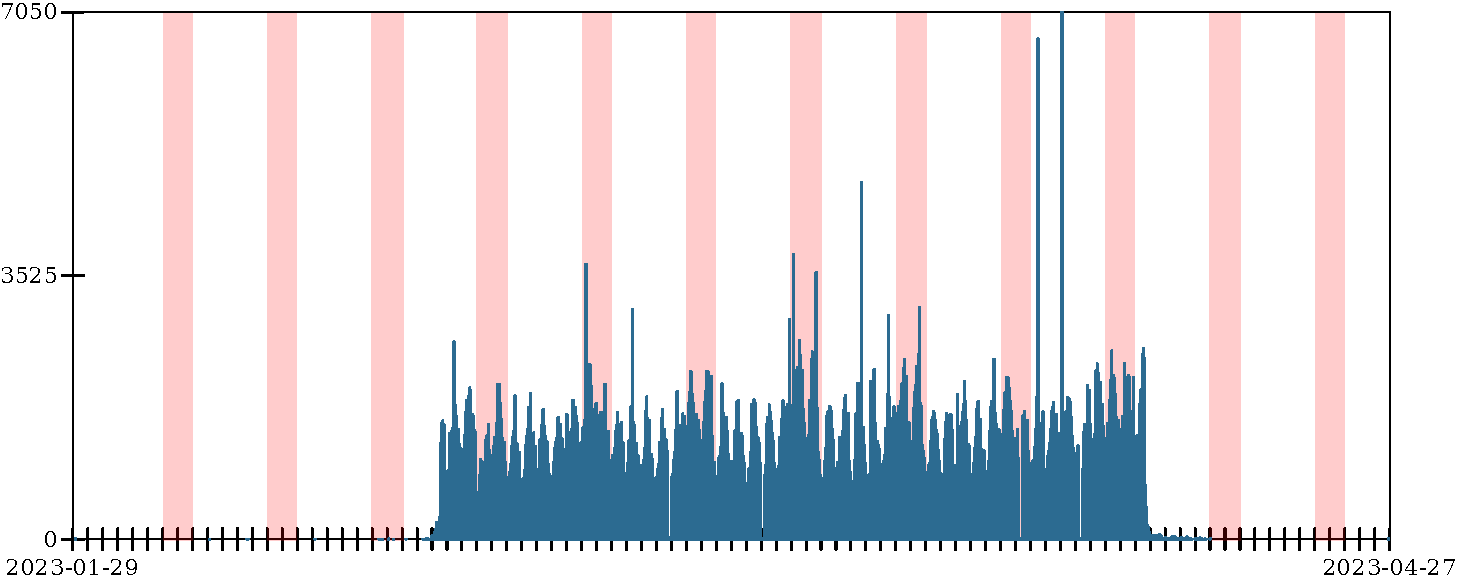
\includegraphics[width=\columnwidth]{img/row-distribution.pdf}
  \caption{Telemetry records per hour. Each tick on the $x$-axis marks the start of a new day in California. Shaded ranges correspond to weekends.}
  \label{f:records-per-hour}
\end{figure}

\begin{figure}[t]
  TODO file size distribution: table or bars %% 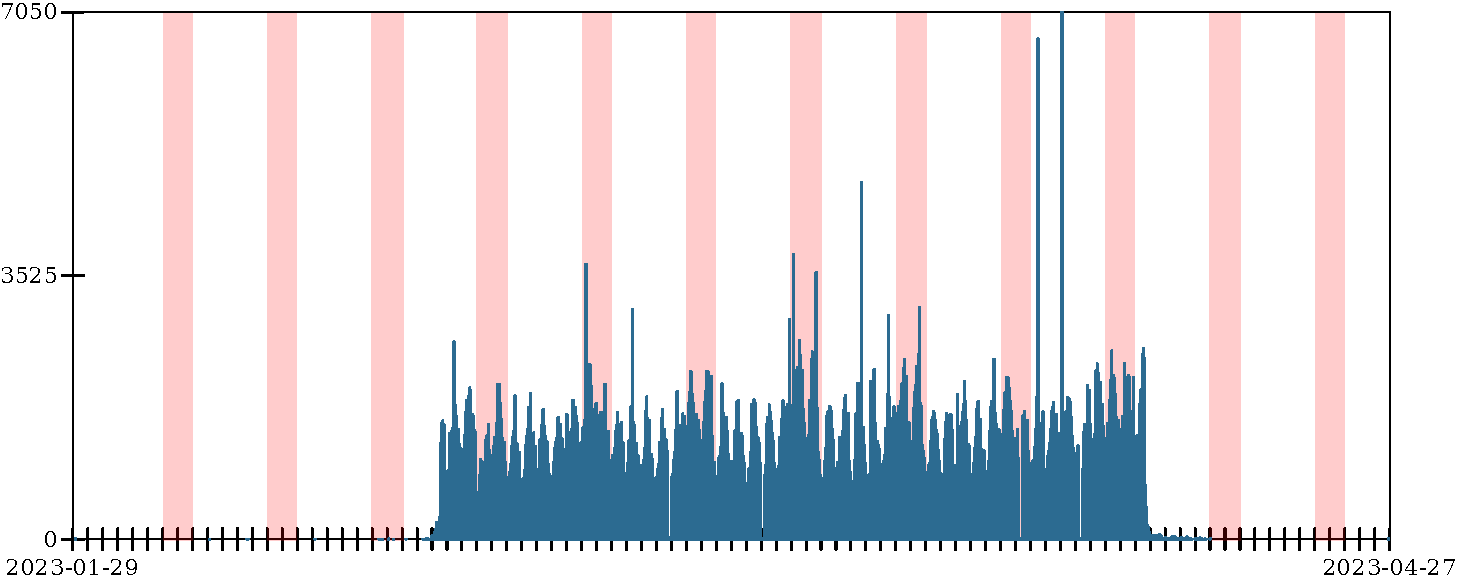
\includegraphics{img/row-distribution.pdf}
  \caption{Size of analyzed code: number of files, number of lines , and lines in edit range}
  \label{f:analysis-size}
\end{figure}


\Cref{f:records-per-hour} shows when data arrived across the whole dataset.
FILL: currently clientTimestamp, which has caveats.
Unclear what timezone they are from.
Some records have a client timestamp much older than the server, up to 1 week behind.
Some are ahead of the server by a day.
Why?
Could be wrong local settings on the computer, or a delayed record due to lost
internet connection or closed laptop.

FILL te in edit range, 
 14,917 non-stx
 16,007 syntax in edit ranges.
 Most are typos!

\begin{figure}[t]
  \begin{subfigure}[t]{\columnwidth}
    \begin{tabular}[t]{ll}
      \begin{tabular}[t]{r@{~~}l@{~~}r}
         1,341,348 & \mnocheck{}          & [\pct{89.14}] \\
           156,883 & \mnonstrict{}        & [\pct{10.43}] \\
             6,505 & \mstrict{}           & [\pct{ 0.43}]
      \end{tabular}
      \begin{tabular}[t]{r@{~~}l@{~~}r}
           508,572 & due to module switch & [\pct{33.80}] \\
           996,164 & due to keystrokes    & [\pct{66.20}]
      \end{tabular}
    \end{tabular}
    \caption{Total telemetry records (1,504,736), analysis modes, and reason-for-sending}
    \label{f:total-records}
  \end{subfigure}

  \begin{subfigure}[t]{\columnwidth}
    \begin{tabular}[t]{ll}
      \begin{tabular}[t]{lrl}
        595,137 & Type errors \\
        289,698 & in current module & [\pct{48.68}] \\
         30,924 & in edit range & [\pct{5.20}]
      \end{tabular}
      \begin{tabular}[t]{lrl}
        72,235,735 & {Forced-strict errors} \\
        37,027,281 & in current module & [\pct{51.26}] \\
         1,111,178 & in edit range & [\pct{1.54}]
      \end{tabular}
    \end{tabular}
    \caption{Type errors and forced-strict errors across all telemetry records}
    \label{f:total-tefs}
  \end{subfigure}

  \begin{subfigure}[t]{\columnwidth}
    \begin{tabular}[t]{ll}
      \begin{tabular}[t]{lrl}
        313,509 & \mnocheck{}   & [\pct{90.19}] \\
         32,902 & \mnonstrict{} & [\pct{ 9.47}] \\
            545 & \mstrict{}    & [\pct{ 0.16}] \\
            642 & mixed-mode    & [\pct{ 0.18}]
      \end{tabular}
      \begin{tabular}[t]{l@{~~}ll}
        \zerowidth{Among the mixed-mode sessions:} \\
        & 341 & contain a mode upgrade \\
        & 320 & contain a mode downgrade \\
        & 512 & contain modules with different modes
      \end{tabular}
    \end{tabular}
    \caption{Total sessions (347,598), whether/how they switch analysis mode}
    \label{f:total-sessions}
  \end{subfigure}

  \caption{Dataset overview}
  \label{f:dataset-overview}
\end{figure}

%% TODO power-law: event count, timespan, files lines editRange /session, 
%% ... gotta know project size

%% results 1 section?!

%% TODO counting stats on type errors
%% - specific errors
%% - typos vs rest
%% - too complex
%% - mod switch vs other

%  %% TODO these need to be plots, it's too much reading for the quick takeaway
%  %% put exactly this data into bars!
%  \begin{minipage}[t]{0.5\textwidth}
%    \begin{tabular}{rr}
%      Session length & \# Sessions \\\midrule
%      1 &  450 \\
%      2 &  199 \\
%      3 &  129 \\
%      4 &  73 \\
%      5 &  60 \\
%      6-10 & 150 \\
%      11-20 & 67 \\
%      21-40 & 11 \\
%      >40 & 7
%      %% max 393
%    \end{tabular}
%  \end{minipage}\begin{minipage}[t]{0.5\textwidth}
%    \begin{tabular}{rr}
%      Time delta & \# Records \\\midrule
%      0-5ms & 284 \\
%      5-1000ms & 248 \\
%      1-2s & 153 \\
%      2-5s & 232 \\
%      5-10s & 207 \\
%      10-30s & 524 \\
%      30-60s & 392 \\
%      1-2m & 394 \\
%      2-5m & 559 \\
%      5-10m & 360 \\
%      >10-60m & 502
%    \end{tabular}
%  \end{minipage}


\begin{figure}[t]
  %% TODO stacked bars?
  %% TODO align old;curr
  \begin{tabular}{lrrrrr}
    Mode             & \# Rows & E         & Any Error & In Module & In range \\
      & & & & (old ; curr) &  (old ; curr) \\\midrule
    \mnocheck{}   &   4,471 & \code{te} &    5.77\% &  0.20\% ;  2.21\% &  0.16\% ;  0.63\% \\
                  &         & \code{fs} &   59.18\% & 32.81\% ; 49.16\% &  9.17\% ; 13.13\% \\
    \mnonstrict{} &     506 & \code{te} &   25.89\% & 12.06\% ; 18.18\% &  6.32\% ;  7.91\% \\
                  &         & \code{fs} &   62.45\% & 37.94\% ; 53.75\% & 16.60\% ; 20.75\% \\
    \mstrict{}    &      24 & \code{te} &   50.00\% & 29.17\% ; 33.33\% &     0\% ;     0\% \\
                  &         & \code{fs} &   62.50\% & 50.00\% ; 58.33\% &  4.17\% ;  8.33\% 
  \end{tabular}

  \bigskip

  Below, edit range only.
  Each record with an edit range error adds +1 to at least 1 row.

  \smallskip

  %% TODO draw bars or curves b/c numbers are too hard to compare horizontally
  \begin{tabular}{lrrr}
    Error Label & \# Add & \# Keep & \# Remove \\\midrule
    CodeTooComplex
    & 0 & 0 & 0 \\
    UnificationTooComplex
    & 0 & 0 & 0 \\[1ex]
    SyntaxError
    & 30 & 0 & 76 \\
    UnknownSymbol
    & 12 & 14 & 19 \\
    UnknownProperty
    & 3 & 1 & 4 \\
    UnknownRequire
    & 1 & 5 & 0 \\
    GenericError
    & 1 & 0 & 1 \\
    CountMismatch
    &  1 &  0 &  1 \\
    OptionalValueAccess
    &  0 &  0 &  1 \\
  \end{tabular}

  \caption{Errors overview}
  \label{f:errors-overview}
\end{figure}

\Cref{f:dataset-overview}:
cannot filter syntax errors from the total and per-module error counts (\cref{s:threats});
multi-mode project = found a module switch that coincides with a mode switch, which suggests that two modules have different modes;
upgrade = found a up-mode switch that does not match a module switch (quite possible to miss these);
downgrade = found a down-mode switch that does not match a module switch

\begin{figure}[t]

  {Few local adds => Few people ignoring script analysis}
  \smallskip

  \begin{tabular}{lrrrr}
    & Local Remove & Local Add & Nonlocal Remove & Nonlocal Add \\
    Mode
    & \#err (\#log)
    & \#err (\#log)
    & \#err (\#log)
    & \#err (\#log) \\\midrule
    \mnocheck{}   & 86 (71) & 0 (0) & 110 (57) & 161 (74) \\
    \mnonstrict{} & 87 (25) & 9 (3) & 185 (29) & 207 (37) \\
    \mstrict{}    &  1  (1) & 0 (0) &  14  (6) &   6  (3) \\
  \end{tabular}

  \caption{Per-mode comparison}
  \label{f:mode-errors}
\end{figure}

\subsection{Analysis 2}

TODO work this into the above or below.

What can we learn from the telemetry? We have 1.5 million records from Feb 22
to April 14 (roughly 27K records per day).
They mention +70 million type errors.
(Some records point to a large number of errors. FILL median, max. Could be cascading,
which makes the 70million number uninterpretable.)
What takeaways are there??!

First,
users rarely switch type analysis mode. There are 3 modes available and users
are free to switch between them, or to mix modes in a codebase, but we rarely
detect these events:

\pct{99} of sessions use a single mode

\pct{0.2} of sessions use different modes in different modules. (More
precisely, the user switched to a module --- triggering a telemetry record ---
that used a different mode than the previous one.)

\pct{0.2} of records show a mode switch (equally split between upgrades and
downgrades, 341 and 320)


Second,
the stronger analysis modes are roughly 10x less popular than weaker ones
(across the \pct{99} of sessions that stick with one mode):

\pct{90} of sessions use nocheck mode
\pct{9.8} use nonstrict mode
\pct{0.2} use strict mode

Third,
In the edit range, we know exactly which errors showed up. This leads to a few
takeaways, such as:

Only 3 sessions (out of +300K) hit the typechecker's internal limits on problem
size --- CodeTooComplex errors. Good!

About \pct{90} of type errors are probably due to typos (SyntaxError, UnknownSymbol,
UnknownProperty). These are not propoer type errors.

10 errors never showed up. These include DynamicPropertyLookupOnClassesUnsafe and
SwappedGenericTypeParameter


Fourth,
Codebase size and session length tend to follow a power law. 
One aspect of size for nonstrict sessions: the number of
lines in the edit range. Over 80 sessions have 20-line ranges, about 40 have a
30-line range, etc.

TODO must explain edit range carefully.

TODO must show full plot, zoomed plot side by side

Fifth,
Increases and decreases to the number of type errors are evenly balanced across
the data.
In strict mode, \pct{24} of records increase the number of type errors. \pct{26}
decrease. \pct{50} keep it constant.
In nonstrict mode, \pct{14} increase errors, \pct{15} decrease, and \pct{71}
keep it constant
This plot is for nonstrict. X-axis = time since start of session, cut off at 30
seconds. Y-axis = change in num errors since last record, cut off at +/- 100.

\begin{figure}[t]
  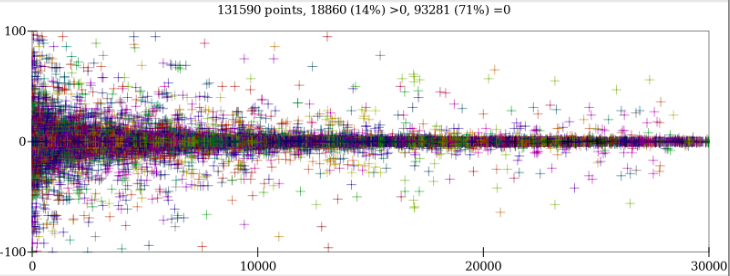
\includegraphics[width=0.8\columnwidth]{img/example-error-delta.png}
  \caption{Errors delta, nonstrict}
  \label{f:error-delta}
\end{figure}

Sixth, a mystery. May be a bug in Luau.
May be DM insensitivity in strict mode
(if DM has top type that would lead to errors.)
Context: each of the 3 modes runs 2 kinds of type analysis. One is the regular
type analysis. The other is Forced Strict (FS), which converts all dependencies
to strict mode. The reason for FS is that it sometimes gives better
autocomplete suggestions etc.
You'd expect that the number of type errors is always <= num FS errors. But we
found several cases where this is false!
The plot here "stacks" every strict session into bars. X-axis is a record index
within a session (bars are higher on the left because we have lots more short
sessions than long ones). Y-axis counts the number of records where num TE <= num FS
is true (blue) and false (yellow).

TODO clarify semantic x-axis order

%% FS has: 1 all dependencies in strict, 2 data-model awareness (DM turns into
%% type graph, ... initial DM, all properties go into a table type; DM -> folder
%% -> model -> part .. get dot-driven autocomplete) in strict, DM might have type
%% Any might have type Instance, the latter would mean more errors than FS

\begin{figure}[t]
  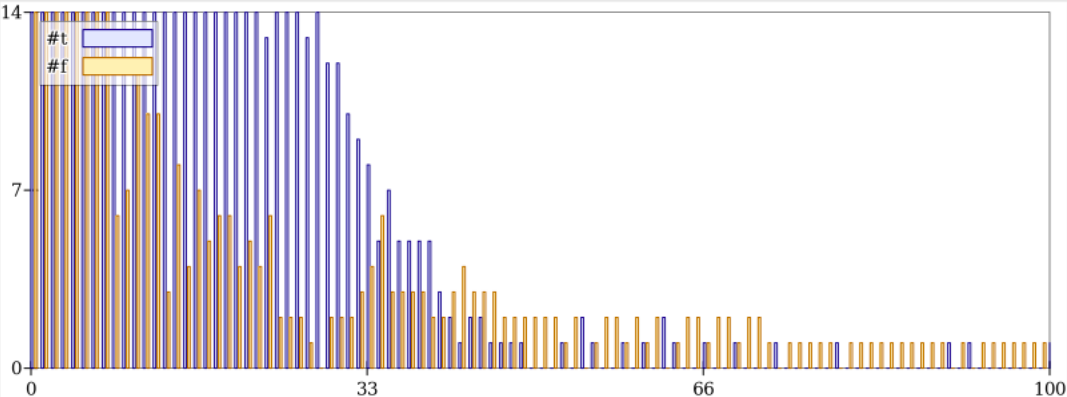
\includegraphics[width=0.8\columnwidth]{img/example-tefs.png}
  \caption{Are there fewer type errors than forcedstrict errors? Expect true always, but that is not the case.}
  \label{f:tefs}
\end{figure}

Seventh, 


\begin{figure}[t]
  \includegraphics[width=0.8\columnwidth]{img/example-compass.png}
  \caption{Are there fewer type errors than forcedstrict errors? Expect true always, but that is not the case.}
  \label{f:tefs}
\end{figure}


\section{Interpretation}

\subsection{Dead Ends: Too Complex}
%% data = out/ctc-info.txt

To deal with pathologies such as the worst-case time for ML-style type
inference~\cite{m-popl-1990,ktu-caap-1990}, the typechecker
has two internal limits to restrict the problems it will attempt to solve.
Hitting a limit triggers either a \code{CodeTooComplex} or
\code{UnificationTooComplex} error.
A casual user should never see these errors.

Fortunately, the data rarely contains too-complex errors.
There are zero \code{UnificationTooComplex} errors and only a
handful of \code{CodeTooComplex} errors.
%% 26 total
It is entirely possible that the \code{CodeTooComplex} errors came from
a single user, as they appear in eleven records (out of 1.5 million)
spread across three sessions.
At any rate, the overall number is low enough to suggest that the internal
limits are not posing barriers to typechecker adoption.


\subsection{TBD}

Error 1000 = type mismatch (subtyping etc);
1001 = unknown symbol;
\ldots

% https://github.com/Roblox/luau/blob/master/Analysis/include/Luau/Error.h


\begin{verbatim}
 require(foobar)
  foobar is a module script in the data model
 require(foo.bar.b)
  - could be edit in progress
  - could be renamed module
  - 
\end{verbatim}


\subsection{Module Switches}

FILL why study, what implications?

FILL need \%s out of all module switches.

How many module switches exit a module with errors?
\mnocheck{} 24, \mnonstrict{} 9, \mstrict{} 3.
Rare?
More common for forcedstrict:
 \mnocheck{} 190, \mnonstrict{} 16, \mstrict{} 2.

How many module switches go to a module with errors?
\mnocheck{} 70, nonstrict 9, strict 4
For FS: \mnocheck{} 400, \mnonstrict{} 39, \mstrict{} 6.


\subsection{Types and Quality of Life}

FILL error density: number vs range size

\begin{figure}[h]
  \begin{tabular}{llrrr}
    Mode & E & Add & Keep & Remove \\\midrule
    \mnocheck{}   & \code{te} & - & - & - \\
                  & \code{fs} & - & - & - \\
    \mnonstrict{} & \code{te} & 16 & 18 & 21 \\
                  & \code{fs} & 19 & 18 & 18 \\
    \mstrict{}    & \code{te} & - & - & - \\
                  & \code{fs} & - & - & - \\
  \end{tabular}

  \caption{Does mode influence the change in total error count?}
  \label{f:edit-deltas}
\end{figure}

TODO nocheck accumulated errors?


\subsection{Example Sessions}

FILL example sessions.

\Cref{f:ex-session-strict} begins in strict mode
but jumps to nocheck mode as well.
The jumps sometimes coincide with module switches (vertical line),
sometimes not.
The green line counts type errors.in the codebase.

\begin{figure}[t]
  \includegraphics[width=0.7\columnwidth]{img/example-session-strict.pdf}
  \caption{Example strict session}
  \label{f:ex-session-strict}
\end{figure}

\Cref{f:ex-session-nonstrict} presents the three sessions from \mnonstrict{} mode
that have the greatest number of events (not necessarily the longest time spans).
There are no module or mode switches.
There are few type errors.
One high point shows 10 errors, but these errors are gone (probably fixed) at
the next event.

\begin{figure}[t]
  \includegraphics[width=0.7\columnwidth]{img/example-session-nonstrict.pdf}
  \caption{Three most populated nonstrict sessions}
  \label{f:ex-session-nonstrict}
\end{figure}

\Cref{f:ex-session-nocheck} shows a roller coaster from \mnocheck{} mode.
Several hundred ForcedStrict type errors appear and disappear between events.
There are lots of module switches too \ldots but that makes no difference
for these project-wide error counts.

\begin{figure}[t]
  \includegraphics[width=0.7\columnwidth]{img/example-session-nocheck.pdf}
  \caption{Example nocheck session}
  \label{f:ex-session-nocheck}
\end{figure}


\subsection{Aggregate Sessions}

\begin{figure}[t]
  \includegraphics[width=0.8\columnwidth]{img/fit-nocheck-Force-3.pdf}
  \includegraphics[width=0.8\columnwidth]{img/fit-nonstrict-TypeE-3.pdf}
  \includegraphics[width=0.8\columnwidth]{img/fit-strict-TypeE-3.pdf}
  \caption{Best-fit curves for errors in each mode (\code{fs} for \mnocheck{}, \code{te} for the others)}
  \label{f:scribbles}
\end{figure}

\Cref{f:scribbles} kill this.

\subsection{Asset Creation vs Scripting}

Data model. Point to discussion above.

Big fluctuations in errors.
FS disagrees with TE.
Probably data model!


\section{Threats to Validity}
\label{s:threats}

Error counts per-project and per-module include syntax errors.
Problematic, because syntax errors are uninteresting (easy to fix),
but common, which makes it likely that our per-keystroke telemetry (1/2k) will record them.
Edit range has specific counts.
Next time, we should do that for the other aggregates.

Telemetry cannot replace user studies, as there is no way to measure
creator sentiment, but provide complementary data at scale.


\section{Related Work}
\label{s:related}

Differential privacy for coverage analysis of software traces,
adds noise to traces,
hard because infinitely many traces,
use CFG abstraction of possible behaviors for callgraph analysis,
count sketch data structure~\cite{hlzbr-ecoop-2021}.

other Nasko papers:
https://dblp.org/pid/83/1412.html

%% - zfstt-ieeesensors-2022
%% - lit review, benefits of static types
%%   http://danluu.com/empirical-pl/
%% - thomas kennedy .... generic usage monitoring ascilite 2003
%% - ahmadzadeh elliman higgins iticse 2005
%% - buffardi etal 2014 adaptive and social mechanisms
%% - bddf-icse-2016
%% -  sh edwards and jason snyder icer 2009 comparing effective and ineffective grading platform
%% - murphy etal sigcse 2009 Retina: helping students
%% - ESP workshop on empirical studies of programming
%%   https://dl.acm.org/doi/proceedings/10.1145/266399
%%   nothing sounds big ... empirical yes, large no
%% - Choppella Haynes IU TR 426
%% - Tip Dinesh tosem 2001

\cite{bgimgm-cse-2016}
study Java compiler error messages after an intervention, counting num errors,
counting repeats, counting per user

\cite{anna-russo-kennedy-ms-2006}
BitFit, web-based java ide log num hint requests num, result of check answer
requests num compile, num run, no code?! good we have the same constraint

\cite{ab-sigcse-2015}
frequency, time-to-fix, spread of errors
 (we can't do time)
parsing compile error + source code
 sometimes with custom parsers

\cite{m-masters-2016}
study errors in blackbox dataset,
 overwhelmingly syntax

\cite{bkmu-sigcse-2014}
blackbox, 100k users
source code, diffs
error line, column, message;
keep all comments EXCEPT one above the class declaration


\cite{bask-icer-2018}
2TB data, Java programs
18 publications survey, technical challenges in analysis
 most pubs analyze errors;
nobody asked:
 which exns do students encounter (what?! mccall kolling 2014)
 execution / editing timelines
(blackbox analysis tutorial in sigcse 2020 on a mini dataset, to help researchers start writing an analysis)


\cite{t-hatra-2021}
plan for a large user-centered study 
... not very deep, look at edit sequences, replay for errors


\cite{cdhhjklwya-hatra-2020}
evaluating the PLIERS design process (Coblenz etal 202X)
teaching students to use PLIERS; everyone ran a user study!
6 languages
 3 ran usability studies
recommend talk-alouds


\cite{gstf-hatra-2021}
liquid types for java
30 devs user study
 zoom

\cite{lfgc-pldi-2007}
typechecker never errors,
 calls a helper that looks for nearby programs that do typecheck
tested on
 10 students, 2yrs professional experience
 5 hw assignments
 2122 files collected;
won \pct{19}, lost \pct{17};
ill-suited for things like (let x = e1 in ....),
 change e1,
 use typechecker feedback to guide edits;
small data!


\cite{w-popl-1986}
reporting source, not detection
tested on 9 type errors
 all \emph{deletions}, such as forgetting to inject in an enum

\cite{sscwj-oopsla-2017}
NATE numerical analysis of type errors
5000 labeled programs
 errors from class, first fix


\cite{sjw-jfp-2018}
type error witness generation
4500 ill-typed student programs
 \pct{85} of time, synthesis works
 \pct{70} of time, locate source


\cite{h-dissertiation-2005}
constraint-based type inference;
general te criteria:
- target audience (novice / expert)
- output format (text / viz)
- interactivity (yes / no)
- heuristics (yes / no)
- primary-or-external (most type errors are easy, some could really use dedicated help)


\cite{hw-scp-2004}
location of type error as a slice,
 not a srcloc,
 not a subtree



\paragraph{Research on Errors}

TODO Liblit dissertiation

Mind your language~\cite{mfk-onward-2011}.


\paragraph{Telemetry}

\begin{table}[t]
  \caption{Comparing telemetry systems}
  \label{t:telemetry-design}

  \begin{tabular}{l@{~}cccccc}
    &             & PII       & Session ID & Deterministic & Private Data \\\midrule
    & Transparent & \chkNo    & \chkNo     & \chkYes       & \chkNo      \\
  * & Us          & \chkNo    & \chkYes    & \chkNo        & \chkYes     \\
    & \code{.NET} & \chkMaybe & \chkYes    & \chkYes       & \chkYes     \\
    & VS Code     & \chkYes   & \chkYes    & \chkYes       & \chkYes     \\
  \end{tabular}
\end{table}

Transparent telemetry: explain what it is and contrast our approach.
What essential, non-transparent things did we collect?

counting only, public decisions about what to count, public data,
collected weekly for a sample of clients, LastWeek field = prior day when
system gathered any data;
eg command invocations, lib stack frames, 
no user ID, no machine ID,
no time-ordered traces~\cite{transparent-telemetry}.

kindle track every tap (page turn etc),
enables whispersync feature,
drove design of navigation tools,
opt-out possible~\cite{kindle-telemetry}

vscode: usage data, crash reports, error data (not a crash but unexpected);
save file, open terminal, copy-paste, autocomplete offered, git queries, machine id,
session id, timestamp,
opt-out may be possible, but not for all usage data (per license, sec 2a) and
every extension can do its own thing~\cite{vscode-telemetry}

.NET SDK and .NET CLI:
crash reports, command invoked, args, hashed cwd, timings;
more listed online;
custom builds beware inadvertant disclosure, keep your filepaths clear;
data published in aggregate under CC-BY;
opt-out possible~\cite{dotnet-telemetry}


\cite{lnsmc-usenix-2018} blame-proportional logging,
scale up ``near'' points of interest,
could be useful for us in the future.
\cite{fnm-sigmod-2020} ditto, faster than statistical at finding root-cause,
deterministic.



\section{Discussion}
\label{s:conclusion}
\label{s:discussion}

FILL regrets, lessons learned, advice for next time



\acks

Greenman was supported by
grant \href{https://nsf.gov/awardsearch/showAward?AWD_ID=2030859&HistoricalAwards=false}{2030859}
to the CRA for the \href{https://cifellows2020.org}{CIFellows} project.

\newpage

\appendix

\section{Data Details}

Tips for interpreting the data:

\begin{itemize}
  \item
    Edit ranges are non-negative because we
    implemented the interval arithmetic for them using unsigned integers.
    To filter out negative edit ranges, we removed all ranges
    greater than 4 billion.

  \item
  \item
  \item
\end{itemize}

\newpage

{ \printbibliography }


\end{document}

% Local Variables:
% TeX-engine: luatex
% End:
